\section{Evaluation}
\label{sec:Evaluation}
This section is structured as, for each experiment and setup a detailed explanation and motivation on how and why the experiment is needed followed by the results of that experiment. The experiments are motivated by gathering as much information and results as possible to answer the research questions. The first subsection~\ref{sec:simulated_results} will present the results from experiments with synthetic data where a reference image is available. The second subsection~\ref{sec:eval_spc} will present the result from images reconstructed from the SPC. No perfect reference image is available in those experiments therefore the images will be evaluated against near optimal image, no reference QA and against a state of the art SWIR camera. 



\subsection{Simulated Results}
\label{sec:simulated_results}
In this section the results produces was simulated by using the reconstructing algorithm and measurement matrix described in section~\ref{sec:TV} and \ref{sec:SOWHMM} on high quality images captured with a state of the art SWIR camera. The images captured by the SWIR camera acts as a ideal reference to the reconstructed images. By simulating the result from "ideal" images the reconstruction process gets a benchmark independent of the SPC.


\subsubsection{Reconstruction performance Using reference image}
\label{sec:reconstruction_performance}
In these simulation 21 images captured with a state of the art SWIR camera was reconstructed. The performance of the reconstruction was calculated using PSNR and SSIM for different degree of noise and sub sampling ratios.\\[0.1in]

To reconstruct the images first the measurement vector was created by calculating the inner product between the measurement matrix ${\mathbf{\Phi}}$ and SWIR image $\mathbf{x}$,

\begin{equation}
\mathbf{y}_{IDEAL} = \mathbf{\Phi}\mathbf{x},
\end{equation}  

where $\mathbf{y}_{IDEAL}$ is an ideal measurement vector given $\mathbf{\Phi} \text{ and } \mathbf{x}$. In the next step white Gaussian noise was added to the normalized measurement signal. The added noise represent a simple model of the noise perturbating the signal in the SPC.

\begin{equation}
\mathbf{y}_R = \mathbf{y}_{IDEAL\_NORMALIZED} + \epsilon,
\end{equation}

where $\mathbf{y}_R$ is the measurement vector used when reconstructing the image and the white Gaussian noise $\epsilon$ added was scaled with the standard deviation $\sigma$ between $0 - 0.2$. \\[0.1in] 

To create the graphs in figure~\ref{fig:psnr_3d} and \ref{fig:ssim_3d} this procedure was applied to all 21 images for sub sampling ratio 5\% to 30\% and added noise with standard deviation between $0 - 0.2$. The standard deviation is not increased above $0.2$ because the reconstruction fails at that point. In figure~\ref{fig:noisy} a sample of reconstructed image from one of the SWIR images is presented with different amount of noise and sub sampling ratios.



\todo[]{Describe how the graphs was created}
\begin{figure}[H]
\vspace*{-0.5cm}
\raggedright
\begin{minipage}[h]{0.245\textwidth}
    
\includegraphics[width=1\textwidth]{result/noisy/1.png}
    \subcaption{Refrence image}
    \label{fig:noise_ref}
\end{minipage}\linebreak
\begin{minipage}[t]{0.245\textwidth}
    
\includegraphics[width = \textwidth]{result/noisy/1_5_20.png}
    \subcaption{$\frac{M}{N} = 5\% \text{, } \sigma = 0.2$}
    \label{fig:noise_5_20}
    
\includegraphics[width = \textwidth]{result/noisy/1_5_12.png}
    \subcaption{$\frac{M}{N} = 5\% \text{, } \sigma = 0.12$}
    \label{fig:noise_5_12}
        
\includegraphics[width = \textwidth]{result/noisy/1_5_6.png}
    \subcaption{$\frac{M}{N} = 5\% \text{, } \sigma = 0.06$}
    \label{fig:noise_5_6}
    
\includegraphics[width = \textwidth]{result/noisy/1_5_0.png}
    \subcaption{$\frac{M}{N} = 5\%$}
    \label{fig:noise_5_0}
\end{minipage}
\begin{minipage}[t]{0.245\textwidth}
    
\includegraphics[width = \textwidth]{result/noisy/1_15_20.png}
    \subcaption{$\frac{M}{N} = 15\% \text{, } \sigma = 0.2$}
    \label{fig:noise_15_20}
    
\includegraphics[width = \textwidth]{result/noisy/1_15_12.png}
    \subcaption{$\frac{M}{N} = 15\% \text{, } \sigma = 0.12$}
    \label{fig:noise_15_12}
    
\includegraphics[width = \textwidth]{result/noisy/1_15_6.png}
    \subcaption{$\frac{M}{N} = 15\% \text{, } \sigma = 0.06$}
    \label{fig:noise_15_6}
    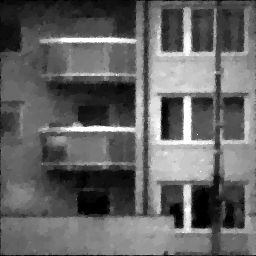
\includegraphics[width = \textwidth]{result/noisy/1_15_0.png}
    \subcaption{$\frac{M}{N} = 15\%$}
    \label{fig:noise_15_0}
\end{minipage}
\begin{minipage}[t]{0.245\textwidth}
    
\includegraphics[width = \textwidth]{result/noisy/1_20_20.png}
    \subcaption{$\frac{M}{N} = 20\% \text{, } \sigma = 0.2$}
    \label{fig:noise_20_20}
    
\includegraphics[width = \textwidth]{result/noisy/1_20_12.png}
    \subcaption{$\frac{M}{N} = 20\% \text{, } \sigma = 0.12$}
    \label{fig:noise_20_12}
    
\includegraphics[width = \textwidth]{result/noisy/1_20_6.png}
    \subcaption{$\frac{M}{N} = 20\% \text{, } \sigma = 0.06$}
    \label{fig:noise_20_6}
    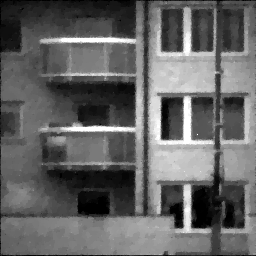
\includegraphics[width = \textwidth]{result/noisy/1_20_0.png}
    \subcaption{$\frac{M}{N} = 20\%$}
    \label{fig:noise_20_0}
\end{minipage}
\begin{minipage}[t]{0.245\textwidth}
    
\includegraphics[width = \textwidth]{result/noisy/1_30_20.png}
    \subcaption{$\frac{M}{N} = 30\% \text{, } \sigma = 0.2$}
    \label{fig:noise_30_20}
    
\includegraphics[width = \textwidth]{result/noisy/1_30_12.png}
    \subcaption{$\frac{M}{N} = 30\% \text{, } \sigma = 0.12$}
    \label{fig:noise_30_12}
    
\includegraphics[width = \textwidth]{result/noisy/1_30_6.png}
    \subcaption{$\frac{M}{N} = 30\% \text{, } \sigma = 0.06$}
    \label{fig:noise_30_6}
    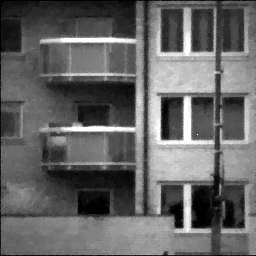
\includegraphics[width = \textwidth]{result/noisy/1_30_0.png}
    \subcaption{$\frac{M}{N} = 30\%$}
    \label{fig:noise_30_0}
\end{minipage}
	\caption{Example of reconstructed images with added noise at different sub sampling ratios.}
	\label{fig:noisy}
\end{figure}

As seen in figure~\ref{fig:noisy} the reconstructed image quality increases with more measurements and lower noise levels. This observation is confirmed in the graphs i figure~\ref{fig:psnr_3d} and \ref{fig:ssim_3d} where PSNR and SSIM respectively has been calculated for all 21 reconstructed images and interpolated. 

\begin{figure}[H]
    \centering
    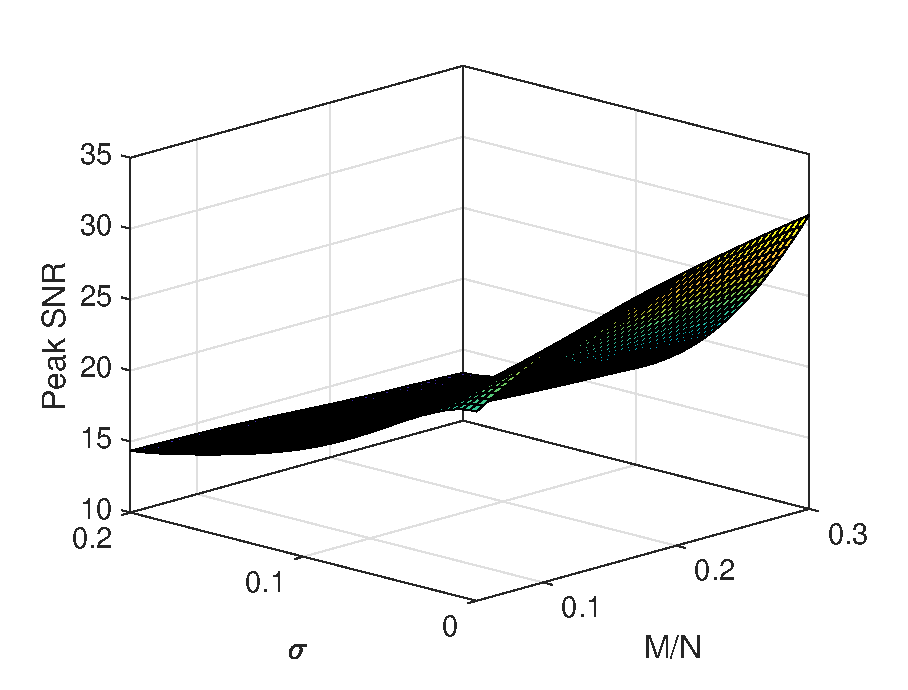
\includegraphics[width = 0.7\linewidth]{result/synt_sss/PSNR_fit.eps}
    \caption{Peak SNR result depending on number of measurements and simulated noise level.}
    \label{fig:psnr_3d}
\end{figure}

\begin{figure}[H]
    \centering
    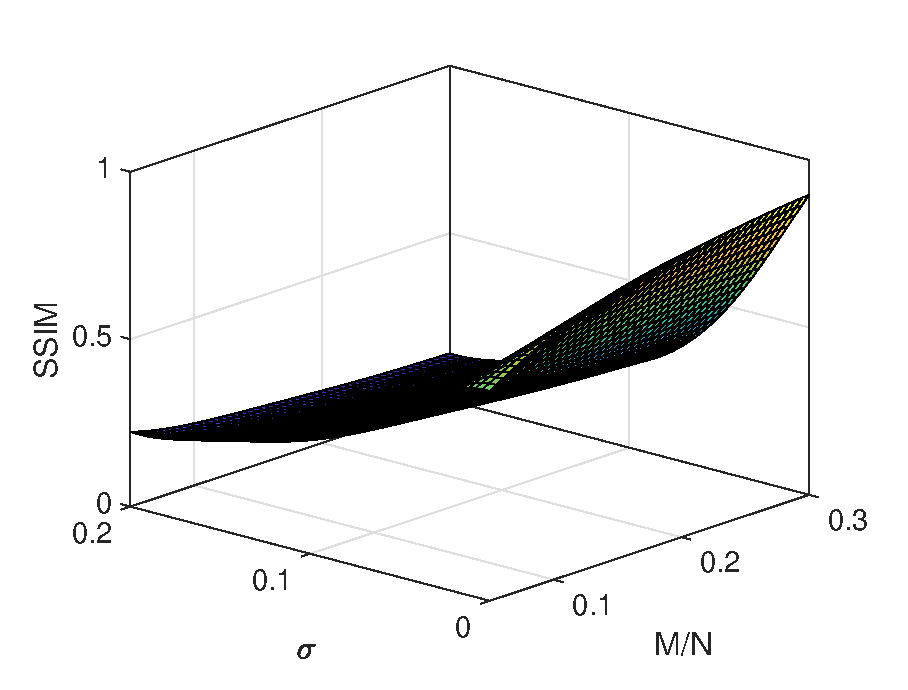
\includegraphics[width = 0.7\linewidth]{result/synt_sss/SSIM_fit.eps}
    \caption{SSIM result depending on number of measurements and simulated noise level.}
    \label{fig:ssim_3d}
\end{figure}

A second observation is that, when the noise increases the  reconstructed image quality is not improved at the same rate as the noiseless case when increasing the sub sampling ratio.

\subsubsection{Reconstruction performance Using no reference quality assessment}
In this sub section the same reconstructed image set from section~\ref{sec:reconstruction_performance} is used to calculate the no reference image quality with the BRISQUE algorithm. This is the same algorithm which will be used to evaluate the results from the SPC therefore this experiments will yield a benchmark on how good results that can be obtained given the measurement matrix and reconstruction algorithm.\\[0.1in] 

The results displayed in the graph in figure~\ref{fig:Brisque_3d} shows the same trend as the results from the previous section, less noise and more samples yields better performance in the reconstruction. The figure also contain the mean results from the original SWIR images as the flat blue surface, which has scored a far superior score than the reconstructed images.
  

\begin{figure}[H]
    \centering
    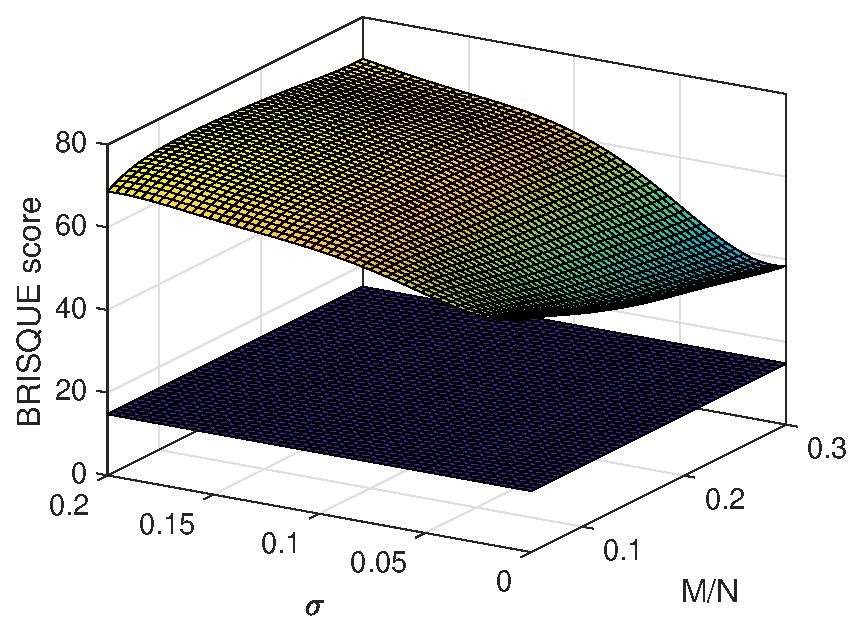
\includegraphics[width = 0.7\linewidth]{result/synt_brisque/BRISQUE_fit.eps}
    \caption{BRISQUE result depending on number of measurements and simulated noise level. Lower surface is reference image score.}
    \label{fig:Brisque_3d}
\end{figure}

In figure~\ref{fig:Brisque_2d} the result has been flatten to a 2D graph with fewer selected data points for clarity. Even in the noiseless case the score will not be better then approximately 40 for the reconstructed images while the SWIR images has a mean value of 15. The conclusion from this result is that, with the current measurement matrix and reconstruction method around 40 in BRISQUE score is what to expect as optimum given that the SPC will induce noise to the signal.   

\begin{figure}[H]
    \centering
    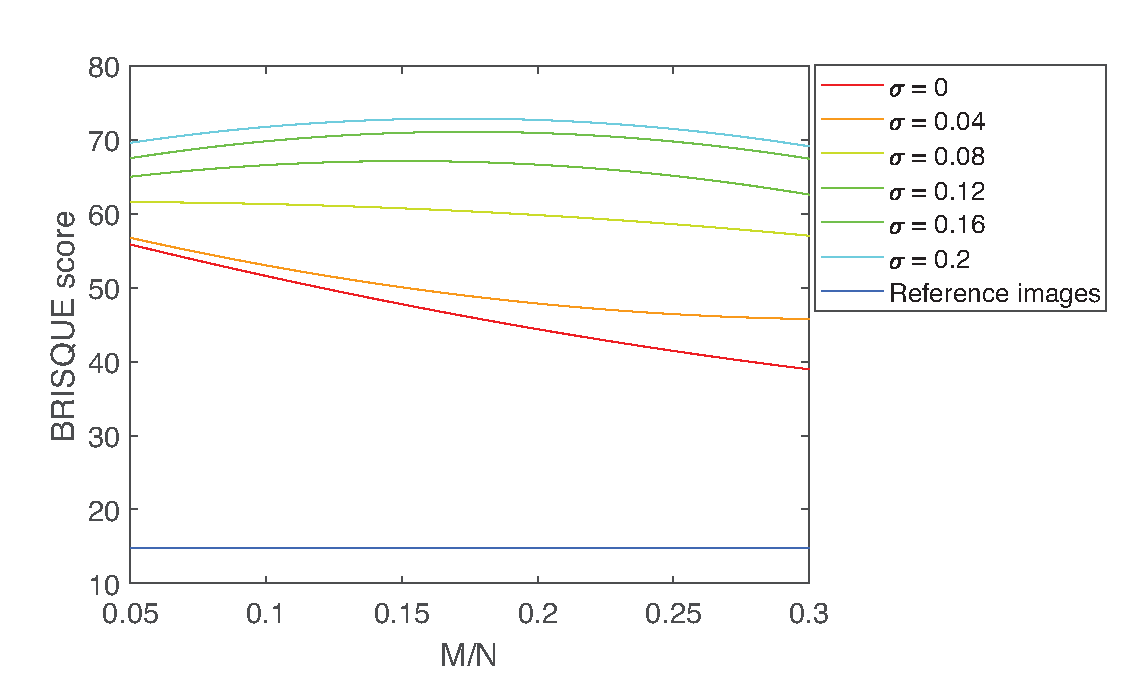
\includegraphics[width = 0.95\linewidth]{result/synt_brisque/Brisque_fit_flat3.eps}
    \caption{BRISQUE result depending on number of measurements for different simulated noise levels.}
    \label{fig:Brisque_2d}
\end{figure}







